\documentclass[11pt,a4paper,openany]{extbook}
\usepackage{tcolorbox}
\usepackage{lipsum}
\usepackage[french]{babel}
\usepackage[T1]{fontenc}
\pagestyle{plain}
\makeatletter
\usepackage{geometry}
\geometry{hmargin=1.5cm,vmargin=1.5cm}
\tcbuselibrary{minted,breakable,xparse,skins}


\setcounter{secnumdepth}{5}% profondeur de la table des matières
\usepackage{titlesec}
\titleformat % design des titres des chapitres
{\chapter}
[display]
{\centering\normalfont\Large\scshape\bfseries}
{\rule[3pt]{0.15\linewidth}{3pt}\quad\thechapter\quad \rule[3pt] {0.15\linewidth}{3pt}}
{0\baselineskip}%espace vertical entre chapitre et nom du chapitre
{\rule{\linewidth}{0.5pt}\break\Huge}
[\vspace{-0.5\baselineskip}\rule{\linewidth}{0.5pt}\vspace{0\baselineskip}]

\definecolor{bg}{gray}{0.95}
\DeclareTCBListing{mintedbox}{O{}m!O{}}{%
  breakable=true,
  listing engine=minted,
  listing only,
  minted language=#2,
  minted style=default,
  minted options={%
    linenos,
    gobble=0,
    breaklines=true,
    breakafter=,,
    fontsize=\small,
    numbersep=8pt,
    #1},
  boxsep=0pt,
  left skip=0pt,
  right skip=0pt,
  left=25pt,
  right=0pt,
  top=3pt,
  bottom=3pt,
  arc=5pt,
  leftrule=0pt,
  rightrule=0pt,
  bottomrule=3pt,
  toprule=3pt,
  colback=bg,
  colframe=orange!70,
  enhanced,
  overlay={%
    \begin{tcbclipinterior}
    \fill[orange!20!white] (frame.south west) rectangle ([xshift=20pt]frame.north west);
    \end{tcbclipinterior}},
  #3}
\begin{document}
\title{\Huge\textbf{Génération et suivi de trajectoire par une voiture autonome}\\ - \\\huge Programmes Python}
\author{\\ \\LÉRONDEL--TOUZÉ Adam, TIPE, Candidat n°23764}
\date{}
\maketitle
\tableofcontents
\chapter{1\up{ères} lignes peu ou prou communes}
\begin{mintedbox}{python}
# -*- coding: utf-8 -*-
"""
Created on Mon Dec 19 19:50:23 2022

@author: adaml
"""


import numpy as np
import matplotlib.pyplot as plt
import matplotlib.animation
import matplotlib.patches
import matplotlib.transforms
import matplotlib.lines
import scipy.interpolate
import shapely
import shapely.geometry
import time
from scipy.integrate import quad as integrale


VITESSE_INIT_VOIT = 5  # vitesse initiale du véhicule
VITESSE_MAX_VOIT = 15  # vitesse maximale (pour rester dans les zones linéaires des modèles)
ACCEL_LAT_MAX = 1.5  # accélération latérale maximale (pour rester dans les zones linéaires des modèles)
LONGUEUR_VEHIC = 5  # longueur du véhicule
LARGEUR_VEHIC = 2  # largeur du véhicule
POSITION_VOITURE_INIT = (-10, -2)  # position (x, y) initiale de la voiture
INCLINAISON_VOITURE_INIT = 0  # inclinaison initiale de la voiture (en degrés)
BRAQUAGE_VOLANT_INIT = 0  # angle volant/voiture en degrés
PRECISION = 15  # nombre de points définissant l'arc de cercle. ie nombre de positions où la voiture ira
TEMPS_REAC = 90  # temps de génération de tentacules
CONE_BRAQUAGE = 0.02  # valeur de braquage définissant des trajectoires "lisses". cf get_tentacules_navigables_et_lisses
COMMENTAIRES = True  # si des commentaires sur l'évolution de l'algo doivent être affichés dans la console
PETIT_POUCET = True  # si on veut récupérer la trajectoire de la voiture
SECURITE = True  # vérifie les collisions. False si aucune sécu, None si check sans arrêter, True si arrêt lorsque collision

# courbure = ro
# courbure = 1/rayon dans le cas d'un cercle
# braquage = delta = arctan(L/rayon) quasi logique (schéma + perpendiculaire)
# longueur = angle*rayon
# empattement +-= longueur voiture


"""
SOME CODE
"""

\end{mintedbox}

\chapter{Affichage des tentacules en arc de cercle}
\begin{figure}[!ht]
    \centering
    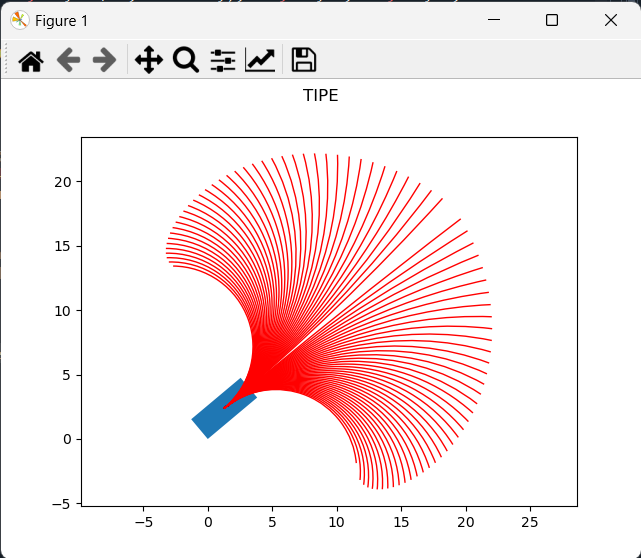
\includegraphics[scale=0.7]{Affichage arcs de cercle.png}
\end{figure}
\vspace{120pt}

\begin{mintedbox}{python}
"""
Affiche la voiture avec ses tentacules en forme d'arcs de cercle.
"""


class Tentacule:
    def __init__(self, voiture, k, delta_k, axes):
        self.axes = axes

        self.L1 = 8 + 72 * (voiture.vitesse/voiture.vitesse_max)**1.2  # formule empirique, équation (9.5) p.123
        # formules pour la longueur p.123 équation (9.4)
        # formules pour le rayon de courbure p.122 équation (9.3)

        if 1 <= k <= 40:  # tentacule à orienter vers la droite
            self.longueur = self.L1 + 20 * np.sqrt((k-1) / 40)
            self.courbure = -np.tan(delta_k) / voiture.longueur

            self.rayon = 1 / self.courbure
            self.angle_rad = self.longueur / self.rayon
            self.angle = self.angle_rad * 180 / np.pi

            self.patch = matplotlib.patches.Arc((voiture.x + self.rayon / 2, voiture.y), self.rayon, self.rayon, theta1=180 - self.angle, theta2=180, color='r')

        elif k == 41:
            self.longueur = self.L1 + 20 * np.sqrt((k-1) / 40)
            self.courbure = 0

            self.patch = matplotlib.patches.Arc((0, 0), 0, 0)

        else:  # 42<=k<=81   # tentacule à orienter vers la gauche
            self.longueur = self.L1 + 20 * np.sqrt((81-k) / 40)
            self.courbure = np.tan(delta_k) / voiture.longueur

            self.rayon = 1 / self.courbure
            self.angle_rad = self.longueur / self.rayon  # en radian
            self.angle = self.angle_rad * 180 / np.pi  # en degrés

            self.patch = matplotlib.patches.Arc((voiture.x - self.rayon / 2, voiture.y), self.rayon, self.rayon, theta1=0, theta2=self.angle, color='r')

        self.patch.set_transform( matplotlib.transforms.Affine2D().rotate_deg_around(voiture.x, voiture.y, voiture.angle - 90) + self.axes.transData)


class Voiture:
    def __init__(self, shape_voiture, x, y, axes):
        self.axes = axes
        self.longueur = LONGUEUR_VEHIC
        self.largeur = LARGEUR_VEHIC
        self.vitesse_max = VITESSE_MAX_VOIT
        self.accel_lat_max = ACCEL_LAT_MAX
        self.shape_voiture = shape_voiture

        self.vitesse = VITESSE_INIT_VOIT
        self.x, self.y = self.shape_voiture.get_center()
        self.angle = INCLINAISON_VOITURE_INIT

        self.courbure_max = self.accel_lat_max / self.vitesse ** 2  # formule p.122 équation (9.1)
        self.braquage_max = np.arctan(self.longueur * self.courbure_max)  # formule p.122 équation (9.2)

        self.transfo_init = self.shape_voiture.get_transform() + matplotlib.transforms.Affine2D().rotate_deg(90)


figure_ref_terre, axes_ref_terre = plt.subplots()
figure_ref_terre.suptitle("TIPE")
simulation_voision_terrestre = Simulation_Ref_Terre()

shape_voiture = matplotlib.patches.Rectangle(POSITION_VOITURE_INIT, LONGUEUR_VEHIC, LARGEUR_VEHIC, INCLINAISON_VOITURE_INIT)
voiture = Voiture(shape_voiture, 0, 0, axes_ref_terre)
axes_ref_terre.add_patch(voiture.shape_voiture)
tentacules = []
deltas = np.linspace(-voiture.braquage_max, voiture.braquage_max, 80)
for k in range(1, 81):
    tentacules.append(Tentacule(voiture, k, deltas[k-1], axes_ref_terre))
for k in range(80):
    axes_ref_terre.add_patch(tentacules[k].patch)


plt.autoscale()
plt.axis('equal')
plt.show()

\end{mintedbox}
\chapter{Affichage des tentacules en forme de clothoïdes}
\begin{figure}[!ht]
    \centering
    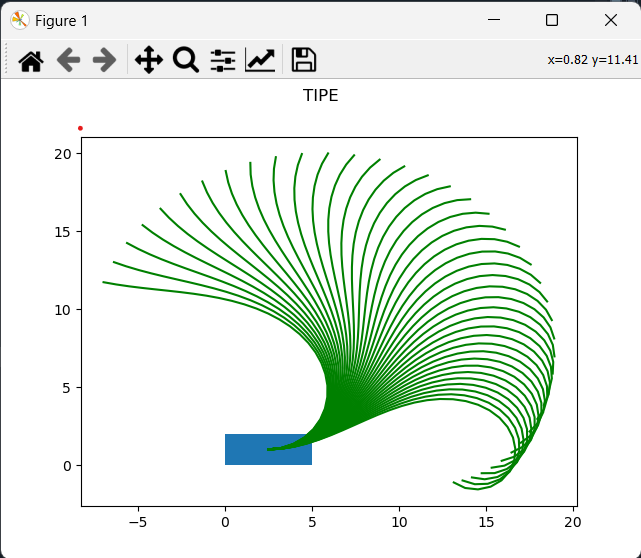
\includegraphics[scale=0.7]{Affichage clotho.png}
\end{figure}
\vspace{120pt}

\begin{mintedbox}{python}
"""Affiche la voiture avec ses tentacules clothoïdaires.
"""


def y(t, rap, ro):
    return integrale(lambda p: np.cos(rap*p**2 + ro*p)/3, 0, t)[0]


def x(t, rap, ro):
    return integrale(lambda p: np.sin(rap*p**2 + ro*p)/3, 0, t)[0]


courbure_tentac_initiale = BRAQUAGE_VOLANT * np.pi / 180


class Tentacule:
    def __init__(self, voiture, rap, ro, axes, L):
        self.voiture = voiture
        self.axes = axes

        self.L = L  # formule empirique, équation (9.15) p.128
        self.precision = PRECISION

        xdata = [x(t, rap, ro) for t in np.linspace(0, int(L), self.precision)]
        ydata = [y(t, rap, ro) for t in np.linspace(0, int(L), self.precision)]
        self.patch = matplotlib.lines.Line2D(xdata, ydata, color='green')
        self.patch.set_transform(matplotlib.transforms.Affine2D().rotate_deg_around(0, 0, voiture.angle - 90) + matplotlib.transforms.Affine2D().translate(voiture.x, voiture.y) + self.axes.transData)


figure_ref_terre, axes_ref_terre = plt.subplots()
figure_ref_terre.suptitle("TIPE")
simulation_voision_terrestre = Simulation_Ref_Terre()

shape_voiture = matplotlib.patches.Rectangle(POSITION_VOITURE_INIT, LONGUEUR_VEHIC, LARGEUR_VEHIC, INCLINAISON_VOITURE_INIT)
voiture = Voiture(shape_voiture, 0, 0, axes_ref_terre)
axes_ref_terre.add_patch(voiture.shape_voiture)
tentacules = []

L = 7*VITESSE_INIT_VOIT - 5  # formule empirique, équation (9.15) p.128
ro_max = ACCEL_LAT_MAX / VITESSE_INIT_VOIT**2
distance_collision = VITESSE_INIT_VOIT**2 / 2*ACCEL_LAT_MAX

rap_min = (-ro_max - courbure_tentac_initiale) / (distance_collision/2)
rap_max = (+ro_max - courbure_tentac_initiale) / (distance_collision/2)
deltas = np.linspace(rap_min, rap_max, 40)
for rap in deltas:
    tentacules.append(Tentacule(voiture, rap, courbure_tentac_initiale + rap*L, axes_ref_terre, L))
for k in range(40):
    axes_ref_terre.add_line(tentacules[k].patch)

plt.autoscale()
plt.show()

\end{mintedbox}

\chapter{Dernières lignes peu ou prou communes}
\begin{mintedbox}{python}
"""
SOME CODE
"""


# création figure + axes
figure_ref_terre, axes_simu = plt.subplots()
figure_data, (axes_vitesse, axes_braquage) = plt.subplots(2, 1, sharex=True)
# titre
figure_ref_terre.suptitle("Animation")
figure_data.suptitle("Données en temps réel")
axes_vitesse.set_title("Vitesse")
axes_braquage.set_title("Braquage")
axes_braquage.set_xlabel("Temps")

# création de la forme de la voiture
shape_voiture = matplotlib.patches.Rectangle(POSITION_VOITURE_INIT, LONGUEUR_VEHIC, LARGEUR_VEHIC, fill=False, zorder=float('inf'))
shape_voiture.rotation_point = 'center'
shape_voiture.set_angle(INCLINAISON_VOITURE_INIT)

# création de la voiture
voiture = Voiture(shape_voiture, [axes_simu, axes_vitesse, axes_braquage], Tentacule_clothoïdaire)

# ajout du dessin de la voiture à la figure
axes_simu.add_patch(voiture.shape_voiture)

# création de la forme de l'obstacle
shape_obstacle = matplotlib.patches.Rectangle((30, -2.5), 2, 1.5, fill=True, zorder=float('inf'), color='cyan')
obstacle1 = Obstacle_fixe(shape_obstacle)
axes_simu.add_patch(obstacle1.patch)

# création des bords de route
shape_route_haut = matplotlib.patches.Rectangle((-10, 5), 90, 2)
route_haut = Obstacle_fixe(shape_route_haut)
axes_simu.add_patch(route_haut.patch)

shape_route_bas = matplotlib.patches.Rectangle((-10, -5), 78, 2)
route_bas = Obstacle_fixe(shape_route_bas)
axes_simu.add_patch(route_bas.patch)

shape_route_gauche = matplotlib.patches.Rectangle((68, -45), 2, 42)
route_gauche = Obstacle_fixe(shape_route_gauche)
axes_simu.add_patch(route_gauche.patch)

shape_route_droite = matplotlib.patches.Rectangle((78, -45), 2, 50)
route_droite = Obstacle_fixe(shape_route_droite)
axes_simu.add_patch(route_droite.patch)

# création de la simulation
simulation = Simulation_Ref_Terre([voiture], [obstacle1, route_bas, route_haut, route_droite, route_gauche])

# création et lancement de l'animation
anim = matplotlib.animation.FuncAnimation(figure_ref_terre,
                                          simulation.animer,
                                          init_func=lambda: [voiture.shape_voiture for voiture in simulation.voitures] + [tentacule.patch for tentacule in simulation.new_tentacules] + [tentacule.patch for tentacule in simulation.old_tentacules],
                                          fargs=[],
                                          interval=35,
                                          cache_frame_data=False,
                                          blit=True,
                                          repeat=True)

# création d'un timer
timer = figure_ref_terre.canvas.new_timer(interval=TEMPS_REAC)
if SECURITE is not False:
    timer2 = figure_ref_terre.canvas.new_timer(40)
    timer2.add_callback(simulation.collisions)
    timer2.start()
    simulation.ajout_timer(timer2)
    figure_ref_terre.canvas.mpl_connect('close_event', lambda event: timer2.stop())
# ajout d'une fonction appelée itérativement
timer.add_callback(simulation.gestion_tentac, voiture)
# démarrage du timer
timer.start()

simulation.ajout_anim(anim)
simulation.ajout_timer(timer)
# stop le timer si on ferme la figure (pour éviter qu'une fonction continue de tourner en boucle sans intérêt une fois tout terminé, c'est plutôt mal vu...!)
figure_ref_terre.canvas.mpl_connect('close_event', lambda event: timer.stop())
figure_ref_terre.canvas.mpl_connect('key_press_event', lambda event: (print("Key Pressed"), simulation.pause_replay()))

axes_simu.autoscale()
# axes_simu.set(xlim=(-50, 50), ylim=(-50, 150))
axes_simu.axis('equal')
plt.show()

\end{mintedbox}

\chapter{Déplacement de la voiture sur une tentacule, sans tenir compte des obstacles}
\begin{figure}[!ht]
    \centering
    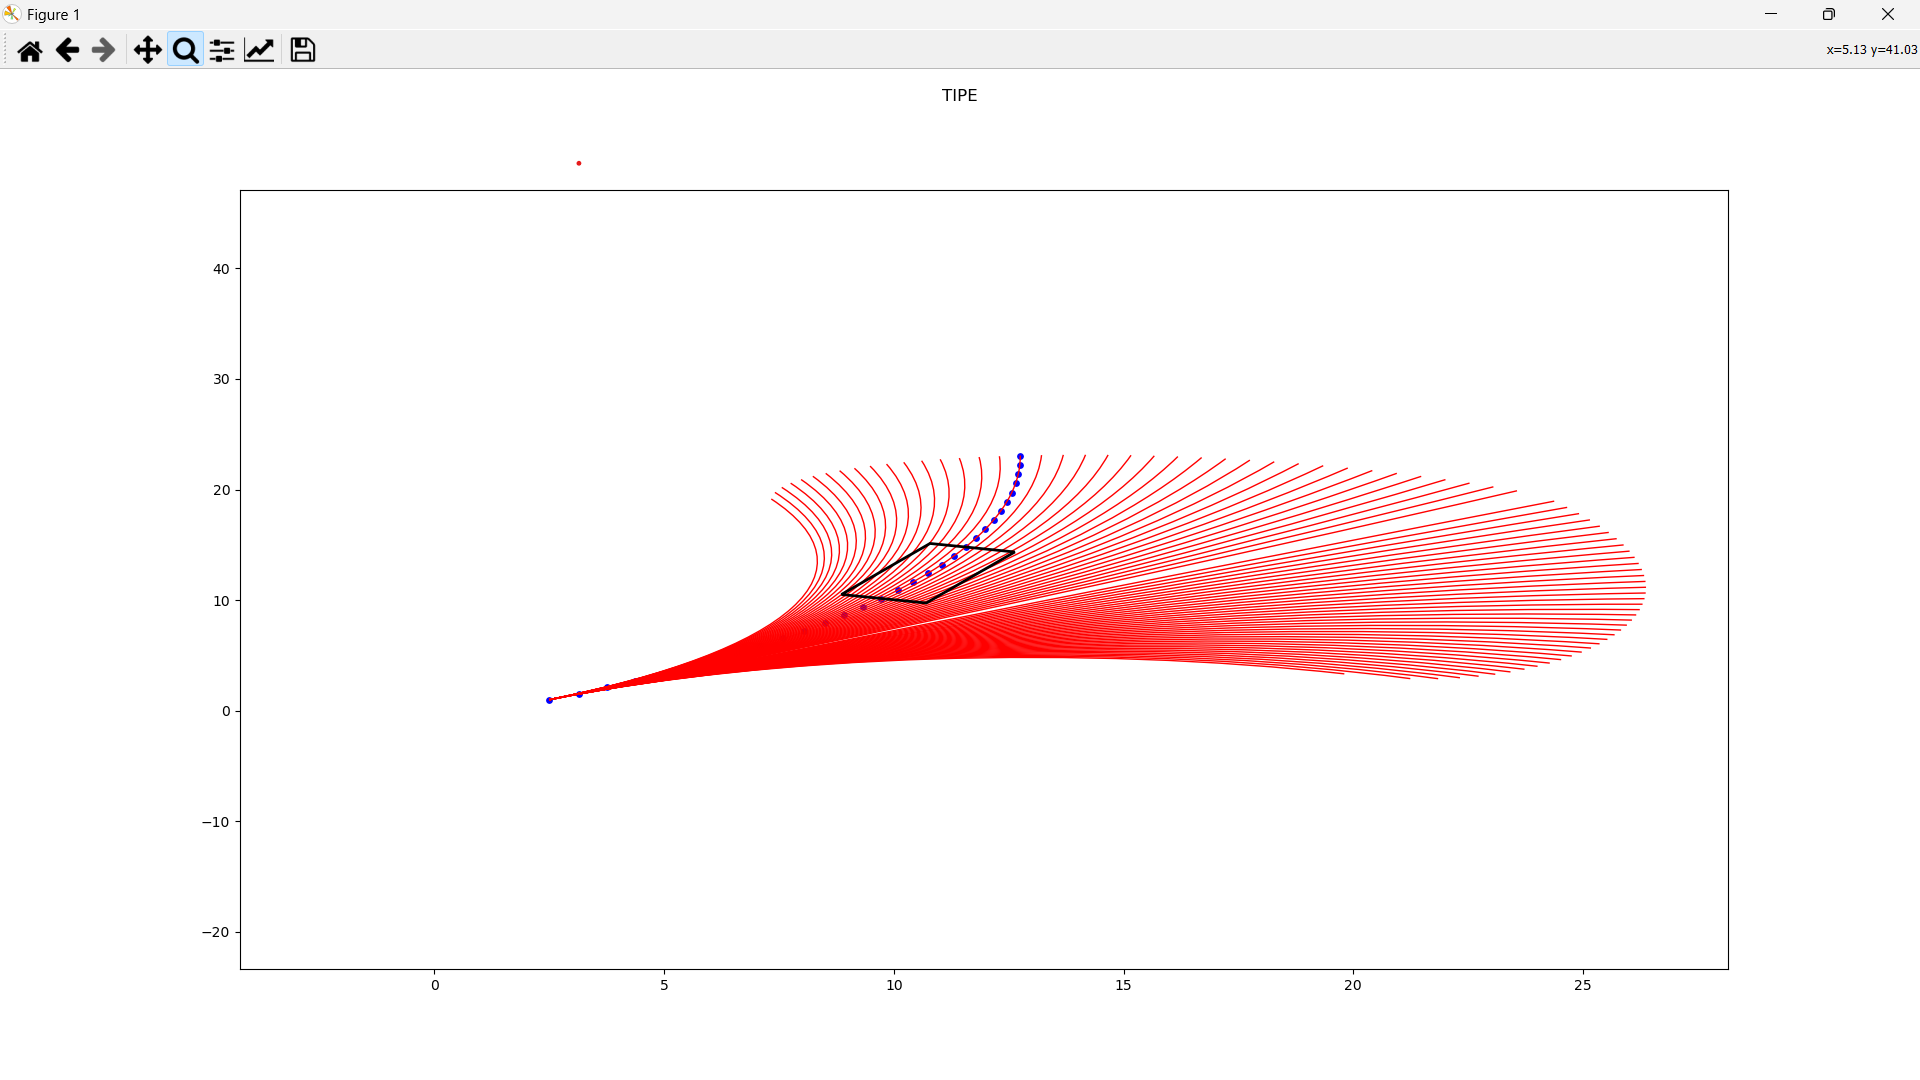
\includegraphics[scale=0.4]{deplacement successifs.png}
\end{figure}
\vspace{100pt}

\begin{mintedbox}{python}
"""
Déplace la voiture indéfiniment (selon une tentacule, puis regénération des tentacules, et suivi, et génération, etc).
"""


class Tentacule:
    """
    Objet tentacule, dépendant d'une voiture, et déterminé par son ordre et son angle de braquage.
    """
    def get_parametric(self, arc=True):
        self.precision = PRECISION
        if arc is True:
            # Définition d'un arc avec un nombre de points contrôlé
            self.patch._path = matplotlib.patches.Path.arc(self.angle_debut, self.angle_fin, self.precision)
        # Paramétrisation de la tentacule
        self.chemin = (self.patch.get_transform() - axes_ref_terre.transData).transform_path( self.patch.get_path()).cleaned().vertices[:-1][::self.signe]
        if arc is False:
            # Interpolation du chemin
            self.chemin_interpol = scipy.interpolate.interp1d(self.chemin[:, 0], self.chemin[:, 1])
            lch = len(self.chemin[:, 0])
            # Interpolation de x(t) pour faire une génération d'abscisses supplémentaires
            points = scipy.interpolate.interp1d(range(0, (lch)*self.precision, self.precision), self.chemin[:, 0])  # va jusque (lch-1)*precision inclus
            # Génération des abscisses supplémentaires avec le points(range) et des ordonnées interpolées correspondantes avec le chemin_interpol(x)
            self.chemin = np.array([[x, self.chemin_interpol(x)] for x in points(range(0, (lch-1)*self.precision, lch-1))])
        return self.chemin


class Voiture:
    """
    Objet voiture, défini par sa forme. D'autres paramètres fixes sont définis après, on pourra les mettre en paramètre plus tard si plusieurs voitures il y a.
    """
    def deplace(self):
        """
        S'il existe un chemin (suite de points), déplace la voiture suivant ce chemin.

        Raises
        ------
        erreur
            Le chemin à suivre n'est pas défini.

        Returns
        -------
        None.

        """
        try:
            new_x = self.chemin[1][0]
            new_y = self.chemin[1][1]
            vx = new_x - self.chemin[0][0]
            vy = new_y - self.chemin[0][1]
            new_angle = np.degrees(np.arctan2(vy, vx))
            self.shape_voiture.set(x=new_x - self.largeur/2, y=new_y - self.longueur/2, angle=new_angle)
            self.x, self.y, self.angle = new_x, new_y, new_angle
            self.chemin = np.delete(self.chemin, 0, 0)
        except IndexError as erreur:
            print('TENTACULE ÉPUISÉE, ON NE SAIT PLUS QUEL CHEMIN SUIVRE')
            # raise erreur

    def update_chemin(self, arc=True):
        """
        Met à jour le chemin que la voiture doit emprunter, en définissant et paramétrant la tentacule.

        Returns
        -------
        None.

        """
        self.remove_tentacules()
        self.generation_tentacules()

        ptch = self.tentacules[NUMERO_DE_LA_TENTACULE].patch  # Récupération de la forme
        self.precision = PRECISION
        if arc is True:
            # Définition d'un arc avec un nombre de points contrôlé
            ptch._path = matplotlib.patches.Path.arc(self.tentacules[NUMERO_DE_LA_TENTACULE].angle_debut, self.tentacules[NUMERO_DE_LA_TENTACULE].angle_fin, self.precision)
        # Paramétrisation de la tentacule
        self.chemin = (ptch.get_transform() - axes_ref_terre.transData).transform_path( ptch.get_path()).cleaned().vertices[:-1][: :self.tentacules[NUMERO_DE_LA_TENTACULE].signe]
        if arc is False:
            # Interpolation du chemin
            self.chemin_interpol = scipy.interpolate.interp1d(self.chemin[:, 0], self.chemin[:, 1])
            lch = len(self.chemin[:, 0])
            # Interpolation de x(t) pour faire une génération d'abscisses supplémentaires
            points = scipy.interpolate.interp1d(range(0, (lch)*self.precision, self.precision), self.chemin[:, 0])  # va jusque (lch-1)*precision inclus
            # Génération des abscisses supplémentaires avec le points(range) et des ordonnées interpolées correspondantes avec le chemin_interpol(x)
            self.chemin = np.array([[x, self.chemin_interpol(x)] for x in points(range(0, (lch-1)*self.precision, lch-1))])
        self.chemin = self.tentacules[NUMERO_DE_LA_TENTACULE].get_parametric()
        # Affichage des points que la voiture devra suivre
        plt.scatter(x=self.chemin[:, 0], y=self.chemin[:, 1], color='b', s=8)

    def generation_tentacules(self):
        """
        Génère les 80 tentacules que la voiture aura la possibilité d'emprunter.

        Returns
        -------
        None.

        """
        self.tentacules = []
        deltas = np.linspace(-self.braquage_max, self.braquage_max, 80)  # 80 est un nombre empirique de tentacules défini dans la thèse (il est bon compromis entre précision et temps de calcul)
        for k in range(1, 81):
            self.tentacules.append(Tentacule(self, k, deltas[k-1], self.axes))  # Ajout de la tentacule aux tentacules appartenant au véhicule
        for k in range(80):
            self.axes.add_patch(self.tentacules[k].patch)  # Ajout de la tentacule à la figure

    def remove_tentacules(self):
        """
        Enlève les tentacules (qui appartiennent au véhicule) de la figure.

        Returns
        -------
        None.

        """
        for tentacule in self.tentacules:
            tentacule.patch.set(visible=False)  # car si simple remove, on perd les axes de référence et c pas bon pour le blit...


class Simulation:
    """
    Classe qui gère tout l'aspect simulation : animation + gestion des objets.

    Parameters
    ----------
    voitures: list
        Liste des voitures présentes
    obstaces: list  # TODO
        liste des obstacles FIXES. Ils ne seront pas animés
    obstacles_mvt: list  # TODO
        liste des obstacles à déplacer. Fonction dévelopée plus tard
    """

    def __init__(self, voitures=[], obstacles_fixes=[], obstacles_mvt=[]):
        self.voitures = voitures
        self.obstacles_fixes = obstacles_fixes
        self.obstacles_mvt = obstacles_mvt
        self.new_tentacules = []  # liste des tentacules à afficher (blit)
        self.old_tentacules = []  # liste des tentacules qui ne sont plus d'actualité, mais qui doivent être supprimées (blit)

        for voitures in self.voitures:
            self.gestion_tentac(voiture)  # créé les tentacules de la voiture, et créé un chemin à suivre (surement inexistants jusqu'alors...)

    def animer(self, i):
        """
        Anime la figure. S'occupe de déplacer les voitures et les obstacles.
        Note : fait appel au "task-manager des tentacules" pour savoir quoi actualiser dans la figure (blit)

        Parameters
        ----------
        i : int
            Numéro d'appel de la fonction (elle est censée être appelée itérativement par une matplotlib.animation.

        Returns
        -------
        list of artists
            Liste des dessins à actualiser (blit).

        """
        # Déplace les voitures
        for voiture in self.voitures:
            voiture.deplace()
        # Déplace les obstacles
        for obstacle in self.obstacles_mvt:
            obstacle.deplace()
        try:
            # Retourne la liste des dessins à actualiser dans la figure
            # TODO : ajouter les obstacles lors de l'import de la fonctionnalité
            return [voiture.shape_voiture for voiture in self.voitures] + [tentacule.patch for tentacule in self.new_tentacules] + [tentacule.patch for tentacule in self.old_tentacules]
        finally:
            # Met juste après les valeurs adéquates à jour pour ne plus avoir à redessiner des dessins fixes (blit)
            self.old_tentacules = []  # Suppression des tentacules obsoletes, qu'on a bien effacé avec le return
            for tentac in self.new_tentacules:
                tentac.patch.set_animated(False)  # Dés-anime les nouvelles tentacules (affichées avec le return) : elles ne doivent plus bouger jusqu'à une redfinition de celles-ci
            # PROBLÈME AU NIVEAU DU BLIT : IL SEMBLERAIT QU'ON SOIT OBLIGÉ DE RETOURNER TOUTES LES TENTACULES À AFFICHER, PLUTÔT QU'UNIQUEMENT CELLES À UPDATE...
            # TODO moins urgent : résoudre ce petit problème de blit si on veut gagner un peu de temps (trace inutilement 80 tentacules...)
            # Suppression des nouvelles tentacules de la liste des dessins à actualiser
            # self.new_tentacules = []

    def gestion_tentac(self, voiture):
        """
        "Task-manager des tentacules"... Gère l'ajout et la suppression des tentacules (appartenant à la voiture *voiture*) de la figure.

        Parameters
        ----------
        voiture : Voiture
            objet voiture.

        Returns
        -------
        None.

        """
        for tentac in voiture.tentacules:  # pour mettre à jour et enlever les tentacules qui vont être supprimées
            tentac.patch.set_animated(True)  # Anime les tentacules à supprimer (elles étaient dés-animées) (blit)
            self.old_tentacules.append(tentac)  # ajout à la liste des dessins à actualiser (blit)

        voiture.update_chemin()  # suppression du système actuel de tentacules pour la voiture, puis génération de nouvelles tentacules pour la voiture

        for tentac in voiture.tentacules:  # pour mettre à jour et ajouter les tentacules qui vont être ajoutées
            tentac.patch.set_animated(True)  # anime les tentacules à ajouter (blit)
            self.new_tentacules.append(tentac)  # ajout à la liste des dessins à actualiser (blit)

\end{mintedbox}

\chapter{Caractérisation de la navigabilité d'une tentacule}
\begin{figure}[!ht]
    \centering
    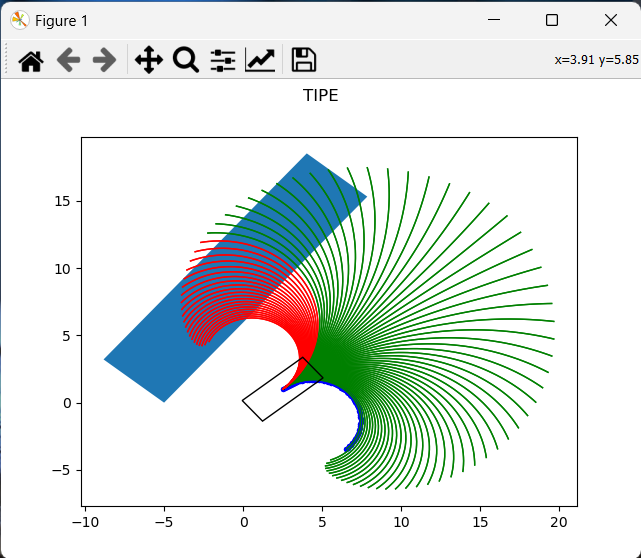
\includegraphics[scale=0.7]{collision.png}
\end{figure}
\vspace{120pt}

\begin{mintedbox}{python}
"""
Trace les tentacules en différentes couleurs, à l'arrêt, selon qu'elles soient navigables ou non.
"""
class Tentacule:
    """
    Objet tentacule, dépendant d'une voiture, et déterminé par son ordre et son angle de braquage.
    """
    def get_zone_support(self):
        if self.voiture.vitesse < 3:
            self.dist_zone_support = 1.4 + 0.2*self.voiture.vitesse/3  # formule empirique p.123 eq(9.6) thèse
        elif 3 <= self.voiture.vitesse <= 15:
            self.dist_zone_support = 1.6 + 0.6 * (self.voiture.vitesse-3) / 15  # idem
        else:
            raise ValueError("La vitesse est trop élevée !")
        self.zone_support = shapely.geometry.LineString( self.get_parametric()).buffer(self.dist_zone_support)
        return self.zone_support

    def is_navigable(self, objets_alentours):
        self.zone_to_be_clean = self.get_zone_support().intersection(self.voiture.get_espace_collision())
        for objet in objets_alentours:
            if objet == self.voiture:  # Pas grave si la tentacule cogne sa propre voiture
                pass
            elif self.zone_to_be_clean.intersection(objet.shapely_poly).is_empty is False:
                self.patch.set_color("red")
                return False
        return True


class Voiture:
    """
    Objet voiture, défini par sa forme. D'autres paramètres fixes sont définis après, on pourra les mettre en paramètre plus tard si plusieurs voitures il y a.
    """
    def get_espace_collision(self):
        self.distance_collision = self.vitesse**2 / 2*self.accel_lat_max
        self.espace_collision = shapely.geometry.Point((self.x, self.y)).buffer(self.distance_collision + self.longueur/2)
        return self.espace_collision

    def is_tentacule_navigable(self, tentacule, objets_alentours):
        return tentacule.is_navigable(objets_alentours)

    def choix_tentacule(self, tentacules_navigables):
        try:
            # On prend la 1ere tentacule lisse qu'on trouve
            for tentacule in tentacules_navigables:
                if tentacule.lisse is True:
                    return tentacule
            # Si aucune n'est lisse, on prend la 1ère
            return tentacules_navigables[0]
        except IndexError:
            raise "AUCUNE TENTACULE NAVIGABLE"

    def get_tentacules_navigables(self, objets_alentours):
        tentacules_navigables = []
        for tentacule in self.tentacules:
            if tentacule.is_navigable(objets_alentours):
                tentacules_navigables.append(tentacule)
        return tentacules_navigables

    def _simu(self, simu):
        self.simu = simu


class Obstacle():
    def __init__(self, patch):
        self.patch = patch
        self.x, self.y = self.patch.get_center()
        self.shapely_poly = shapely.geometry.Polygon(
            (self.patch.get_transform()).transform_path(self.patch.get_path()).vertices)


class Obstacle_fixe(Obstacle):
    def __init__(self, patch):
        super().__init__(patch)

\end{mintedbox}

\chapter{Déplacement en évitant les obstacles (sans choix optimal de tentacule)}
\begin{figure}[!ht]
    \centering
    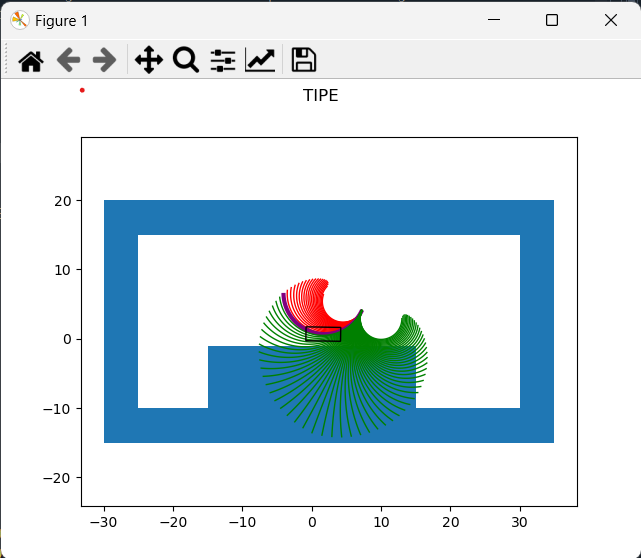
\includegraphics[scale=0.7]{carre.png}
\end{figure}
\vspace{120pt}

\begin{mintedbox}{python}
"""
Déplace la voiture dans une enceinte carrée.
"""
class Voiture:
    """
    Objet voiture, défini par sa forme. D'autres paramètres fixes sont définis après, on pourra les mettre en paramètre plus tard si plusieurs voitures il y a.
    """
    def choix_tentacule(self, tentacules_navigables):
        # TODO : faire un critère de dégagement du tentacule (p. 125 section 9.2.4.1)
        # TODO : faire un critère de changement de braquage (p.125 section 9.2.4.2)
        # TODO moins important car nécessite GPS et tt (pas forcément notre objet d'étude) : faire un critère de rapprochement de la trajectoire globale (p.126 section 9.2.4.3)

        try:
            # On prend la 1ere tentacule lisse qu'on trouve
            for tentacule in tentacules_navigables:
                if tentacule.lisse is True:
                    return tentacule
            # Si aucune n'est lisse, on prend la dernière
            return tentacules_navigables[-1]
        except IndexError:
            raise "AUCUNE TENTACULE NAVIGABLE"

\end{mintedbox}

\chapter{Critère de choix d'une tentacule}
\begin{figure}[!ht]
    \centering
    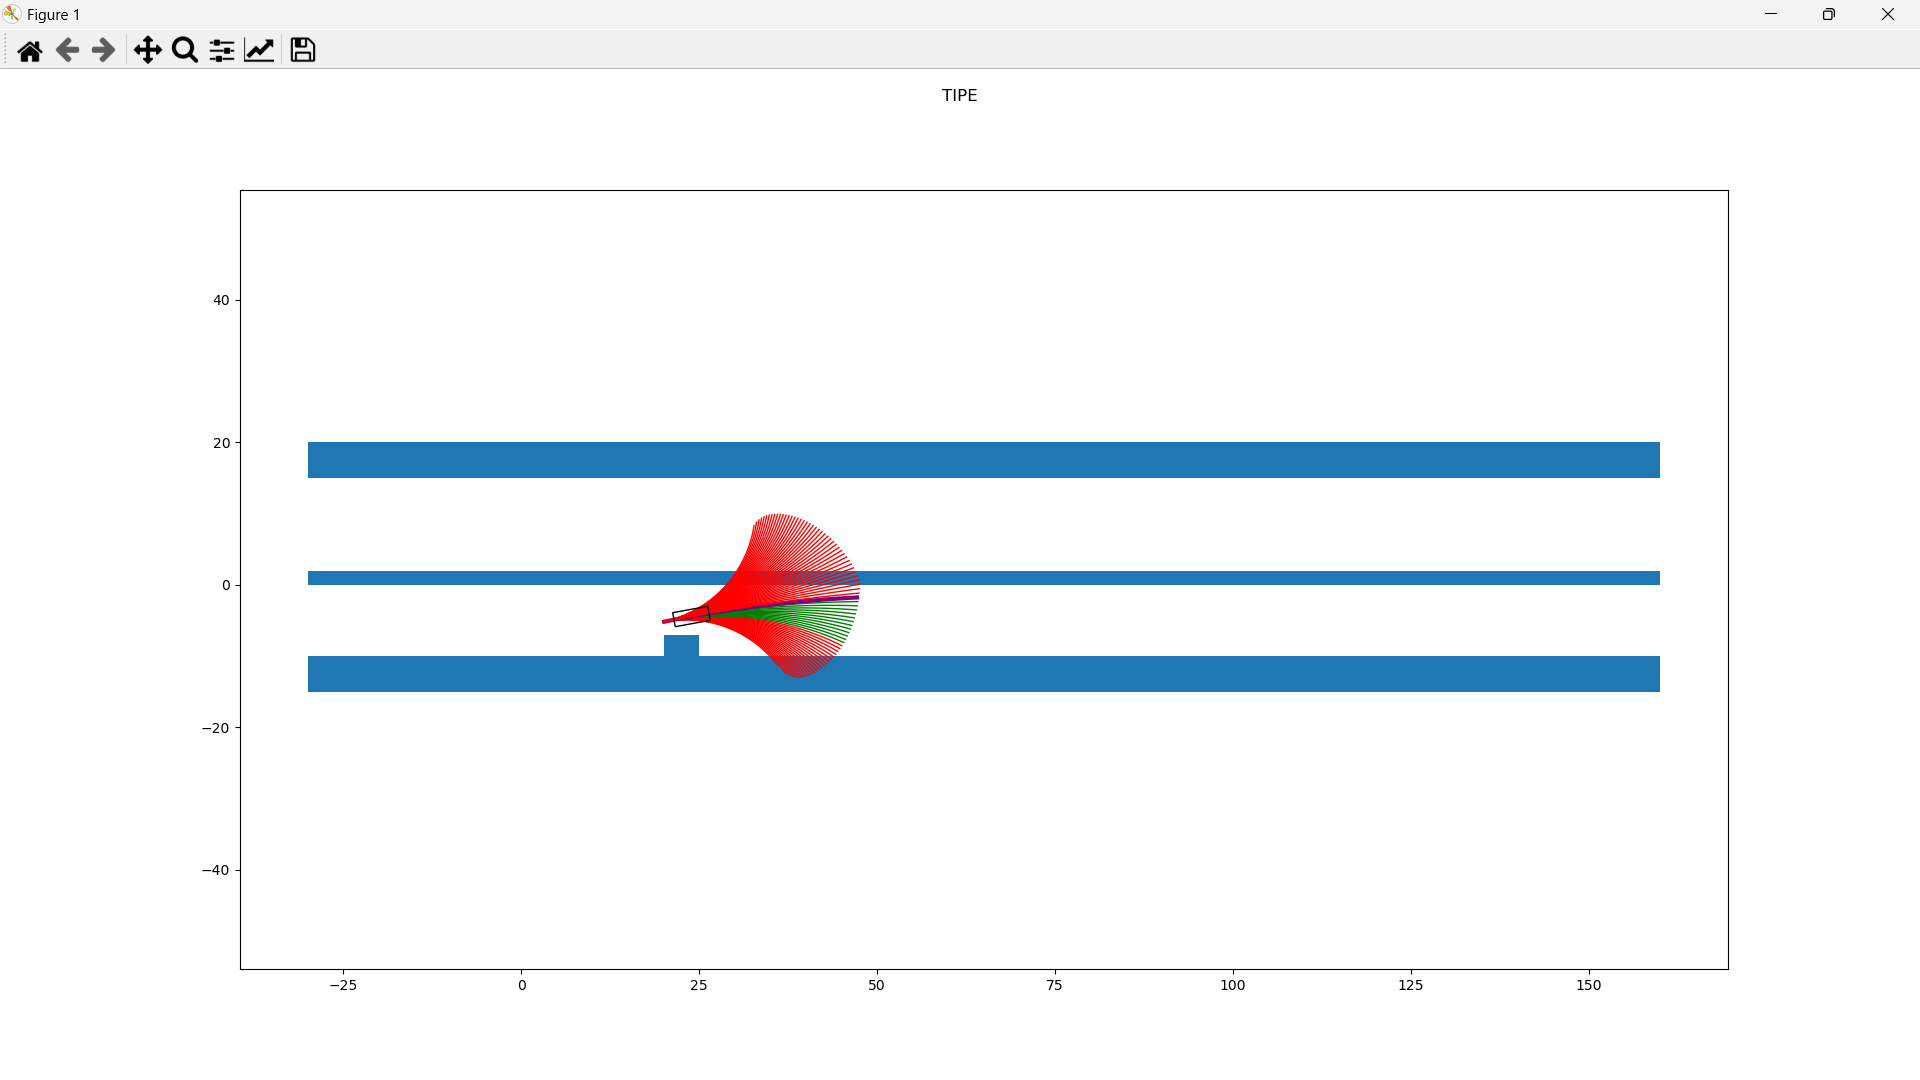
\includegraphics[scale=0.4]{evitement simple.png}
\end{figure}
\vspace{100pt}

\begin{mintedbox}{python}
"""
Déplace la voiture de manière optimal sur un parcours.
"""
class Tentacule:
    """
    Objet tentacule, dépendant d'une voiture, et déterminé par son ordre et son angle de braquage.
    """

    def __init__(self, voiture, k, delta_k, axes):
        self.V_lisse = abs(self.braquage - self.voiture.braquage) / (2 * self.voiture.braquage_max)


class Voiture:
    """
    Objet voiture, défini par sa forme. D'autres paramètres fixes sont définis après, on pourra les mettre en paramètre plus tard si plusieurs voitures il y a.
    """
    def choix_tentacule(self, tentacules_navigables):
        # TODO : faire un critère de dégagement du tentacule (p. 125 section 9.2.4.1)
        # TODO moins important car nécessite GPS et tt (pas forcément notre objet d'étude) : faire un critère de rapprochement de la trajectoire globale (p.126 section 9.2.4.3)

        try:
            return min(tentacules_navigables, key=lambda x: x.V_lisse**4 + x.braquage**2)  # On trie selon une loi fonction de V_lisse (écart au braquage actuel) et de braquage (trajectoire droite). Puis on prend le min
        except ValueError:
            print("AUCUNE TENTACULE NAVIGABLE")

\end{mintedbox}

\chapter{Optimisation de l'algorithme et ajout de "l'houache" de la "voiture"}
\begin{figure}[!ht]
    \centering
    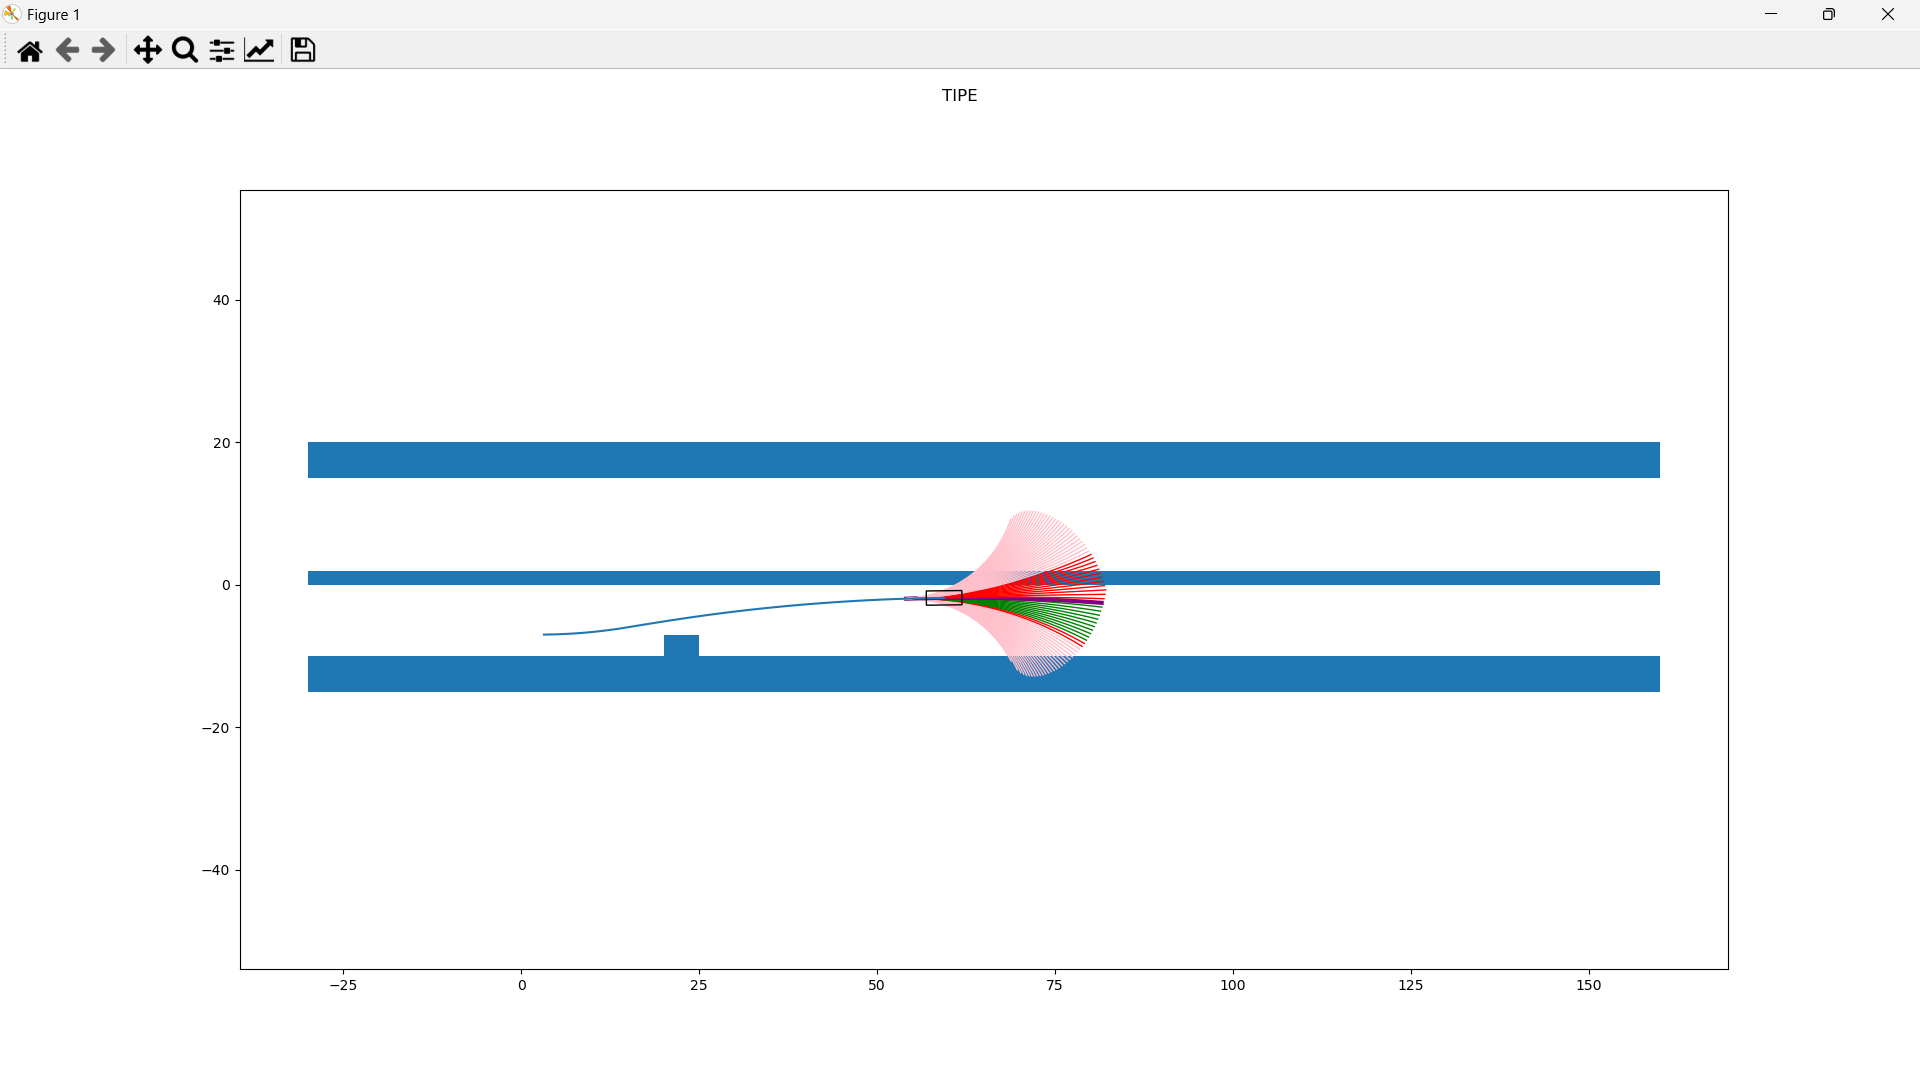
\includegraphics[scale=0.3]{evitement fin.png}
\end{figure}
\vspace{100pt}

\begin{mintedbox}{python}
"""
Déplacement de la voiture sur un parcours, en n'évaluant pas toutes les tentacules (gain de temps) et en affichant la trace de la voiture.
"""


class Voiture:
    """
    Objet voiture, défini par sa forme. D'autres paramètres fixes sont définis après, on pourra les mettre en paramètre plus tard si plusieurs voitures il y a.
    """
    def deplace(self):
        """
        S'il existe un chemin (suite de points), déplace la voiture suivant ce chemin.

        Raises
        ------
        erreur
            Le chemin à suivre n'est pas défini.

        Returns
        -------
        None.

        """
        try:
            new_x = self.chemin[1][0]
            new_y = self.chemin[1][1]
            vx = new_x - self.chemin[0][0]
            vy = new_y - self.chemin[0][1]
            new_angle = np.degrees(np.arctan2(vy, vx))
            self.shape_voiture.set(x=new_x - self.largeur/2, y=new_y - self.longueur/2, angle=new_angle)
            self.x, self.y, self.angle = new_x, new_y, new_angle
            self.chemin = np.delete(self.chemin, 0, 0)
            if self.traceur is True:
                self.trace.set_data(np.append(self.trace.get_data()[0], new_x), np.append(self.trace.get_data()[1], new_y))
        except IndexError:
            print('TENTACULE ÉPUISÉE, ON NE SAIT PLUS QUEL CHEMIN SUIVRE')

class Simulation_Ref_Terre:
    """
    Classe qui gère tout l'aspect simulation : animation + gestion des objets.

    Parameters
    ----------
    voitures: list
        Liste des voitures présentes
    obstaces: list  # TODO
        liste des obstacles FIXES. Ils ne seront pas animés
    obstacles_mvt: list  # TODO
        liste des obstacles à déplacer. Fonction dévelopée plus tard
    """
    def animer(self, i):
        """
        Anime la figure. S'occupe de déplacer les voitures et les obstacles.
        Note : fait appel au "task-manager des tentacules" pour savoir quoi actualiser dans la figure (blit)

        Parameters
        ----------
        i : int
            Numéro d'appel de la fonction (elle est censée être appelée itérativement par une matplotlib.animation.

        Returns
        -------
        list of artists
            Liste des dessins à actualiser (blit).

        """
        traces = []
        # Déplace les voitures
        for voiture in self.voitures:
            voiture.deplace()
        # Déplace les obstacles
        for obstacle in self.obstacles_mvt:
            obstacle.deplace()
        try:
            # Retourne la liste des dessins à actualiser dans la figure
            # TODO : ajouter les obstacles lors de l'import de la fonctionnalité
            return [voiture.shape_voiture for voiture in self.voitures] + [tentacule.patch for tentacule in self.new_tentacules] + [tentacule.patch for tentacule in self.old_tentacules] + [obstacle.patch for obstacle in self.obstacles_mvt] + [voiture.trace for voiture in self.voitures]
        finally:
            # Met juste après les valeurs adéquates à jour pour ne plus avoir à redessiner des dessins fixes (blit)
            self.old_tentacules = []  # Suppression des tentacules obsoletes, qu'on a bien effacé avec le return
            for tentac in self.old_tentacules:
                tentac.patch.remove()
            for tentac in self.new_tentacules:
                tentac.patch.set_animated(False)  # Dés-anime les nouvelles tentacules (affichées avec le return) : elles ne doivent plus bouger jusqu'à une redfinition de celles-ci. Sert ?

\end{mintedbox}

\include{Final version}
\end{document}
